%%%%%%%%%%%%%%%%%%%%%%%%%%%%%%%%%%%%%%%%%%%%%%%%%%%%%%%%%%%%%%%%%%%%
%% %%	Posterdown PDF class for LaTeX files	 08-JAN-2019
%% %%	For any information please send an e-mail to:
%% %%		brentthonre18@gmail.com (Brent Thorne)
%% %%
%% %%	Initial class provided by:
%% %%		Brent Thorne
%% %% Contributors: Shea Connell (SC)
%%%%%%%%%%%%%%%%%%%%%%%%%%%%%%%%%%%%%%%%%%%%%%%%%%%%%%%%%%%%%%%%%%%%

\documentclass[article,30pt,extrafontsizes]{memoir}

%utf-8 seems to be important
\RequirePackage[utf8]{inputenc}
\RequirePackage[T1]{fontenc}
\RequirePackage{lmodern}
\RequirePackage{multicol}
\RequirePackage{graphicx}
\RequirePackage{lipsum}
\RequirePackage{blindtext}
\RequirePackage[svgnames,table]{xcolor}
\RequirePackage{tikz}
\RequirePackage[framemethod=tikz]{mdframed}
\RequirePackage{color}
\RequirePackage{geometry}
\RequirePackage{adjmulticol}
\RequirePackage[skins,most,listings,skins]{tcolorbox}

%For kable extra package :)
\RequirePackage{booktabs}
\RequirePackage{longtable}
\RequirePackage{array}
\RequirePackage{multirow}
\RequirePackage{wrapfig}
\RequirePackage{float}
\RequirePackage{colortbl}
\RequirePackage{pdflscape}
\RequirePackage{pagecolor}
\RequirePackage{tabu}
\RequirePackage{threeparttable}
\RequirePackage{threeparttablex}
\RequirePackage[normalem]{ulem}
\RequirePackage{makecell}
\RequirePackage{wrapfig}

%rof hyperrefs
\RequirePackage{hyperref}
\hypersetup{
    colorlinks=true,
    linkcolor=linkcol,
    citecolor=citecol,
    filecolor=linkcol,
    urlcolor=urlcol,
}
%For figure and table placement
\RequirePackage{float}
\floatplacement{figure}{H}
\floatplacement{table}{H}

%%%%%%%%% COLOURS %%%%%%%%
%Fill/ Line Colours
\definecolor{titleboxbgcol}{HTML}{}
\definecolor{titleboxbordercol}{HTML}{}
\definecolor{columnlinecol}{HTML}{}
\definecolor{bodybgcol}{HTML}{}
\definecolor{sectitlebgcol}{HTML}{}
\definecolor{sectitlebordercol}{HTML}{}
% Text Colours
\definecolor{titletextcol}{HTML}{}
\definecolor{authortextcol}{HTML}{}
\definecolor{affiliationtextcol}{HTML}{}
\definecolor{sectitletextcol}{HTML}{}
\definecolor{bodytextcol}{HTML}{}
\definecolor{footnotetextcol}{HTML}{}
\definecolor{citecol}{HTML}{}
\definecolor{urlcol}{HTML}{}
\definecolor{linkcol}{HTML}{}


%Memoir spacing options
%spacing between figure/ table and caption
\setlength{\abovecaptionskip}{0.4in}
\setlength{\belowcaptionskip}{0.2in}
\captionnamefont{\footnotesize\sffamily\bfseries}
\captiontitlefont{\footnotesize\sffamily}

%define column options
\setlength{\columnseprule}{}
\def\columnseprulecolor{\color{columnlinecol}}

%define section title features
\setsubsubsecheadstyle{\small\color{sectitletextcol}\textbf}% Set \section style
\setsecnumformat{}
\def\sectionmark#1{\markboth{#1}{#1}}

%%%%%%%%%%%% TCOLORBOXES TO THE RESCUE %%%%%%%%%%%%%%%%%%%%
%Title Box
\newtcolorbox{topbox}{
enhanced,
colback=titleboxbgcol,
colframe=titleboxbordercol,
halign=center,
boxrule=,
sharp corners=,
 overlay={
    \node[anchor=south west]
      at ([xshift=,yshift=]frame.south west)
       {\includegraphics[width=]{https://raw.githubusercontent.com/brentthorne/posterdown/master/images/betterhexlogo.png}};
    \node[anchor=south east]
      at ([xshift=,yshift=]frame.south east)
       {\includegraphics[width=]{https://raw.githubusercontent.com/brentthorne/posterdown/master/images/betterhexlogo.png}};}

}
%Body Section Title Box
\newtcolorbox{myboxstuff}[1][]{
code={\parindent=0em},
colframe=sectitlebordercol,
nobeforeafter,
left skip=0pt,
valign=center,
halign=center,
fontupper=\Large\bfseries,
colupper=sectitletextcol,
boxrule=,
colback=sectitlebgcol,
sharp corners=, #1}
\newcommand{\mybox}[1]{%
\begin{myboxstuff}
\strut #1
\end{myboxstuff}%
}
\makeheadstyles{MyBox}{
    \setsecheadstyle{\mybox}
}
\headstyles{MyBox}\makepagestyle{MyBox}
%-----------------------------------------------------
%Make sure that the page is empty of any preset items from memoir
\thispagestyle{empty}

%biblatex options
\RequirePackage[sorting=none,backend=biber]{biblatex}
\renewcommand*{\bibfont}{\} %% SC
\bibliography{packages.bib}
\defbibheading{bibliography}[\bibname]{%
\setlength\bibitemsep{\itemsep} %% SC
\section*{#1}%
\markboth{#1}{#1}}
\AtBeginDocument{%
  \renewcommand{\bibname}{References}
}

%Remove section numbering & set 2nd level header as first level
%to avoid the automatic new page generated from memoir chapter
%formatting
\counterwithout{section}{chapter}
\makechapterstyle{mydefault}{
\addtocounter{secnumdepth}{2}
\setsecheadstyle{\mybox}
\setsubsecheadstyle{\itshape}
\setsubsubsecheadstyle{\itshape}
}

%set the chapterstyle
\chapterstyle{mydefault}

%define column spacing
\setlength\columnsep{}

%spacing params
\setlength\parindent{0em}
\setlength\parskip{0em}
\setlength\hangparas{0}

%spacing after section head title
\setaftersecskip{0em}
\setbeforesecskip{1.5em}
\setlength\textfloatsep{0in}
\setlength\floatsep{0in}
\setlength\intextsep{0in}

\setstocksize{36in}{48in}
\settrimmedsize{\stockheight}{\stockwidth}{*}
\settypeblocksize{36in}{48in}{*}
\setlrmargins{*}{*}{1}
\setulmarginsandblock{2.5cm}{*}{*}
\setmarginnotes{0em}{0cm}{0cm}
\setlength{\footskip}{0cm}
\setlength{\footnotesep}{0cm}
\setlength{\headheight}{0pt}
\setlength{\headsep}{0pt}
\setlength{\trimtop}{0pt}
\setlength{\trimedge}{0pt}
\setlength{\uppermargin}{0pt}
\checkandfixthelayout

%Footnote to white
\RequirePackage{footmisc}
\def\footnotelayout{\centering\color{footnotetextcol}}

% see https://stackoverflow.com/a/47122900

% choose font family
\RequirePackage{}

% define the BODYBGCOL
\newpagecolor{bodybgcol}

%sets footnote to be white hopefully
\renewcommand\footnoterule{}
\renewcommand{\thempfootnote}{\footnotesize\color{footnotetextcol}{\arabic{mpfootnote}}}

%include arbitrary input from header-includes field
\usepackage{booktabs}
\usepackage{longtable}
\usepackage{array}
\usepackage{multirow}
\usepackage{wrapfig}
\usepackage{float}
\usepackage{colortbl}
\usepackage{pdflscape}
\usepackage{tabu}
\usepackage{threeparttable}
\usepackage{threeparttablex}
\usepackage[normalem]{ulem}
\usepackage{makecell}
\usepackage{xcolor}

%-------------- Begin Document -------------------%
\begin{document}

%-------------- Title Box Start ------------------%
%tcolorbox allows for pictures hopefully
\begin{topbox}
  \color{titletextcol}
  \vspace{0.5in}
  \{Intact but Atypical Lexical and Syntactic Alignment in Spontaneous
Speech of Children with Autism Spectrum Disorder}  \\[0.3in]  %% SC
  \color{authortextcol} \{true} \\[0.2in] %% SC
  \color{affiliationtextcol} \{true} %% SC
  \vspace{1cm}
\end{topbox}
%--------------- Title Box End -------------------%
%----------------- Body Start --------------------%
% Begin body of poster
\begin{adjmulticols*}{3}{}{}
\{  %% SC
\color{bodytextcol}
\section{What is Conversational
Alignment?}\label{what-is-conversational-alignment}

\begin{figure}

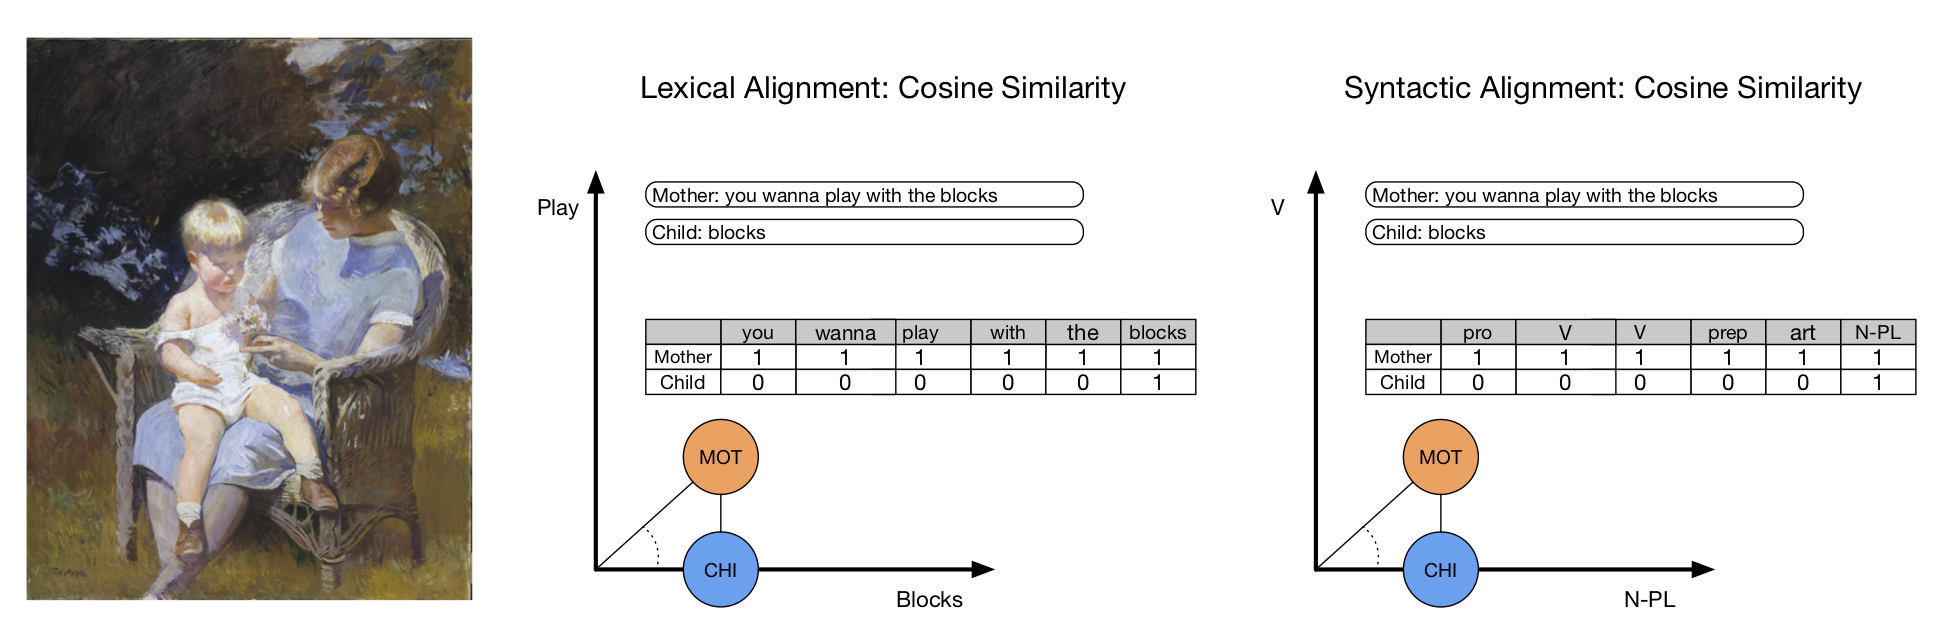
\includegraphics[width=1\linewidth,height=1\textheight]{Cosine-similarity} \hfill{}

\caption{Edmund C. Tarbell, "Marjorie and Little Edmund"}\label{fig:unnamed-chunk-1}
\end{figure}

\section{Do Children Align?}\label{do-children-align}

\begin{table}

\caption{\label{tab:table1}Alignment Rate: Do Children Align?}
\centering
\begin{tabular}[t]{l|l|l}
\hline
Predictors & Lexical & Syntactic\\
\hline
ASD & <span style="display: inline-block; border-radius: 2px; padding-right: 2px; background-color: lightgreen; width: 10.47%; margin-left: 50%; text-align: right;">0.09</span> & <span style="display: inline-block; border-radius: 2px; padding-right: 2px; background-color: lightpink; width: 11.43%; margin-right: 50%; text-align: right; float: right; ">-0.16</span>\\
\hline
Visit & <span style="display: inline-block; border-radius: 2px; padding-right: 2px; background-color: lightgreen; width: 17.44%; margin-left: 50%; text-align: right;">0.15</span> & <span style="display: inline-block; border-radius: 2px; padding-right: 2px; background-color: lightgreen; width: 14.29%; margin-left: 50%; text-align: right;">0.2</span>\\
\hline
Visit * ASD & <span style="display: inline-block; border-radius: 2px; padding-right: 2px; background-color: lightpink; width: 5.81%; margin-right: 50%; text-align: right; float: right; ">-0.05</span> & <span style="display: inline-block; border-radius: 2px; padding-right: 2px; background-color: lightpink; width: 5.71%; margin-right: 50%; text-align: right; float: right; ">-0.08</span>\\
\hline
Vineland Socialization (VS) & <span style="display: inline-block; border-radius: 2px; padding-right: 2px; background-color: lightgreen; width: 50%; margin-left: 50%; text-align: right;">0.43</span> & <span style="display: inline-block; border-radius: 2px; padding-right: 2px; background-color: lightgreen; width: 12.14%; margin-left: 50%; text-align: right;">0.17</span>\\
\hline
VS *ASD & <span style="display: inline-block; border-radius: 2px; padding-right: 2px; background-color: lightgreen; width: 17.44%; margin-left: 50%; text-align: right;">0.15</span> & <span style="display: inline-block; border-radius: 2px; padding-right: 2px; background-color: lightgreen; width: 50%; margin-left: 50%; text-align: right;">0.7</span>\\
\hline
VS * Visit & <span style="display: inline-block; border-radius: 2px; padding-right: 2px; background-color: lightpink; width: 10.47%; margin-right: 50%; text-align: right; float: right; ">-0.09</span> & <span style="display: inline-block; border-radius: 2px; padding-right: 2px; background-color: lightgreen; width: 11.43%; margin-left: 50%; text-align: right;">0.16</span>\\
\hline
Mullen Expressive Language (MEL) & <span style="display: inline-block; border-radius: 2px; padding-right: 2px; background-color: lightgreen; width: 32.56%; margin-left: 50%; text-align: right;">0.28</span> & <span style="display: inline-block; border-radius: 2px; padding-right: 2px; background-color: lightgreen; width: 25.71%; margin-left: 50%; text-align: right;">0.36</span>\\
\hline
MEL * ASD & <span style="display: inline-block; border-radius: 2px; padding-right: 2px; background-color: lightgreen; width: 13.95%; margin-left: 50%; text-align: right;">0.12</span> & <span style="display: inline-block; border-radius: 2px; padding-right: 2px; background-color: lightpink; width: 0%; margin-right: 50%; text-align: right; float: right; ">0</span>\\
\hline
MEL * Visit & <span style="display: inline-block; border-radius: 2px; padding-right: 2px; background-color: lightpink; width: 6.98%; margin-right: 50%; text-align: right; float: right; ">-0.06</span> & <span style="display: inline-block; border-radius: 2px; padding-right: 2px; background-color: lightpink; width: 0%; margin-right: 50%; text-align: right; float: right; ">0</span>\\
\hline
MEL * ASD * Visit & <span style="display: inline-block; border-radius: 2px; padding-right: 2px; background-color: lightgreen; width: 1.16%; margin-left: 50%; text-align: right;">0.01</span> & <span style="display: inline-block; border-radius: 2px; padding-right: 2px; background-color: lightpink; width: 0%; margin-right: 50%; text-align: right; float: right; ">0</span>\\
\hline
\end{tabular}
\end{table}

\section{How Much do Children Align?}\label{how-much-do-children-align}

\begin{table}

\caption{\label{tab:table2}Alignment Level: How Much Do Children Align?}
\centering
\begin{tabular}[t]{l|l|l}
\hline
Predictors & Lexical & Syntactic\\
\hline
ASD & <span style="display: inline-block; border-radius: 2px; padding-right: 2px; background-color: lightpink; width: 47.5%; margin-right: 50%; text-align: right; float: right; ">-0.19</span> & <span style="display: inline-block; border-radius: 2px; padding-right: 2px; background-color: lightgreen; width: 1.79%; margin-left: 50%; text-align: right;">0.02</span>\\
\hline
Visit & <span style="display: inline-block; border-radius: 2px; padding-right: 2px; background-color: lightpink; width: 12.5%; margin-right: 50%; text-align: right; float: right; ">-0.05</span> & <span style="display: inline-block; border-radius: 2px; padding-right: 2px; background-color: lightpink; width: 5.36%; margin-right: 50%; text-align: right; float: right; ">-0.06</span>\\
\hline
Visit * ASD & <span style="display: inline-block; border-radius: 2px; padding-right: 2px; background-color: lightgreen; width: 15%; margin-left: 50%; text-align: right;">0.06</span> & <span style="display: inline-block; border-radius: 2px; padding-right: 2px; background-color: lightgreen; width: 2.68%; margin-left: 50%; text-align: right;">0.03</span>\\
\hline
Vineland Socialization (VS) & <span style="display: inline-block; border-radius: 2px; padding-right: 2px; background-color: lightgreen; width: 10%; margin-left: 50%; text-align: right;">0.04</span> & <span style="display: inline-block; border-radius: 2px; padding-right: 2px; background-color: lightgreen; width: 3.57%; margin-left: 50%; text-align: right;">0.04</span>\\
\hline
VS *ASD & <span style="display: inline-block; border-radius: 2px; padding-right: 2px; background-color: lightpink; width: 0%; margin-right: 50%; text-align: right; float: right; ">0</span> & <span style="display: inline-block; border-radius: 2px; padding-right: 2px; background-color: lightpink; width: 50%; margin-right: 50%; text-align: right; float: right; ">-0.56</span>\\
\hline
VS * Visit & <span style="display: inline-block; border-radius: 2px; padding-right: 2px; background-color: lightpink; width: 2.5%; margin-right: 50%; text-align: right; float: right; ">-0.01</span> & <span style="display: inline-block; border-radius: 2px; padding-right: 2px; background-color: lightgreen; width: 2.68%; margin-left: 50%; text-align: right;">0.03</span>\\
\hline
VS * ASD * Visit & <span style="display: inline-block; border-radius: 2px; padding-right: 2px; background-color: lightpink; width: 0%; margin-right: 50%; text-align: right; float: right; ">0</span> & <span style="display: inline-block; border-radius: 2px; padding-right: 2px; background-color: lightpink; width: 0%; margin-right: 50%; text-align: right; float: right; ">0</span>\\
\hline
Mullen Expressive Language (MEL) & <span style="display: inline-block; border-radius: 2px; padding-right: 2px; background-color: lightpink; width: 5%; margin-right: 50%; text-align: right; float: right; ">-0.02</span> & <span style="display: inline-block; border-radius: 2px; padding-right: 2px; background-color: lightpink; width: 5.36%; margin-right: 50%; text-align: right; float: right; ">-0.06</span>\\
\hline
MEL * ASD & <span style="display: inline-block; border-radius: 2px; padding-right: 2px; background-color: lightgreen; width: 50%; margin-left: 50%; text-align: right;">0.2</span> & <span style="display: inline-block; border-radius: 2px; padding-right: 2px; background-color: lightpink; width: 0%; margin-right: 50%; text-align: right; float: right; ">0</span>\\
\hline
MEL * Visit & <span style="display: inline-block; border-radius: 2px; padding-right: 2px; background-color: lightpink; width: 0%; margin-right: 50%; text-align: right; float: right; ">0</span> & <span style="display: inline-block; border-radius: 2px; padding-right: 2px; background-color: lightpink; width: 0%; margin-right: 50%; text-align: right; float: right; ">0</span>\\
\hline
MEL * ASD * Visit & <span style="display: inline-block; border-radius: 2px; padding-right: 2px; background-color: lightpink; width: 10%; margin-right: 50%; text-align: right; float: right; ">-0.04</span> & <span style="display: inline-block; border-radius: 2px; padding-right: 2px; background-color: lightpink; width: 0%; margin-right: 50%; text-align: right; float: right; ">0</span>\\
\hline
\end{tabular}
\end{table}

\section{How Much of Children's Alignment is Exact
Repetition?}\label{how-much-of-childrens-alignment-is-exact-repetition}

\begin{table}

\caption{\label{tab:table3}Exact Repetitions}
\centering
\begin{tabular}[t]{l|l|l}
\hline
Predictors & Lexical & Syntactic\\
\hline
ASD & <span style="display: inline-block; border-radius: 2px; padding-right: 2px; background-color: lightgreen; width: 7.89%; margin-left: 50%; text-align: right;">0.09</span> & <span style="display: inline-block; border-radius: 2px; padding-right: 2px; background-color: lightgreen; width: 10.67%; margin-left: 50%; text-align: right;">0.16</span>\\
\hline
Visit & <span style="display: inline-block; border-radius: 2px; padding-right: 2px; background-color: lightpink; width: 17.54%; margin-right: 50%; text-align: right; float: right; ">-0.2</span> & <span style="display: inline-block; border-radius: 2px; padding-right: 2px; background-color: lightpink; width: 13.33%; margin-right: 50%; text-align: right; float: right; ">-0.2</span>\\
\hline
Visit * ASD & <span style="display: inline-block; border-radius: 2px; padding-right: 2px; background-color: lightgreen; width: 11.4%; margin-left: 50%; text-align: right;">0.13</span> & <span style="display: inline-block; border-radius: 2px; padding-right: 2px; background-color: lightgreen; width: 5.33%; margin-left: 50%; text-align: right;">0.08</span>\\
\hline
Vineland Socialization (VS) & <span style="display: inline-block; border-radius: 2px; padding-right: 2px; background-color: lightgreen; width: 50%; margin-left: 50%; text-align: right;">0.57</span> & <span style="display: inline-block; border-radius: 2px; padding-right: 2px; background-color: lightgreen; width: 50%; margin-left: 50%; text-align: right;">0.75</span>\\
\hline
VS *ASD & <span style="display: inline-block; border-radius: 2px; padding-right: 2px; background-color: lightpink; width: 32.46%; margin-right: 50%; text-align: right; float: right; ">-0.37</span> & <span style="display: inline-block; border-radius: 2px; padding-right: 2px; background-color: lightpink; width: 46.67%; margin-right: 50%; text-align: right; float: right; ">-0.7</span>\\
\hline
VS * Visit & <span style="display: inline-block; border-radius: 2px; padding-right: 2px; background-color: lightpink; width: 11.4%; margin-right: 50%; text-align: right; float: right; ">-0.13</span> & <span style="display: inline-block; border-radius: 2px; padding-right: 2px; background-color: lightpink; width: 10.67%; margin-right: 50%; text-align: right; float: right; ">-0.16</span>\\
\hline
VS * ASD * Visit & <span style="display: inline-block; border-radius: 2px; padding-right: 2px; background-color: lightpink; width: 0%; margin-right: 50%; text-align: right; float: right; ">0</span> & <span style="display: inline-block; border-radius: 2px; padding-right: 2px; background-color: lightpink; width: 0%; margin-right: 50%; text-align: right; float: right; ">0</span>\\
\hline
Mullen Expressive Language (MEL) & <span style="display: inline-block; border-radius: 2px; padding-right: 2px; background-color: lightpink; width: 49.12%; margin-right: 50%; text-align: right; float: right; ">-0.56</span> & <span style="display: inline-block; border-radius: 2px; padding-right: 2px; background-color: lightpink; width: 31.33%; margin-right: 50%; text-align: right; float: right; ">-0.47</span>\\
\hline
MEL * ASD & <span style="display: inline-block; border-radius: 2px; padding-right: 2px; background-color: lightgreen; width: 35.96%; margin-left: 50%; text-align: right;">0.41</span> & <span style="display: inline-block; border-radius: 2px; padding-right: 2px; background-color: lightpink; width: 0%; margin-right: 50%; text-align: right; float: right; ">0</span>\\
\hline
MEL * Visit & <span style="display: inline-block; border-radius: 2px; padding-right: 2px; background-color: lightgreen; width: 9.65%; margin-left: 50%; text-align: right;">0.11</span> & <span style="display: inline-block; border-radius: 2px; padding-right: 2px; background-color: lightpink; width: 0%; margin-right: 50%; text-align: right; float: right; ">0</span>\\
\hline
MEL * ASD * Visit & <span style="display: inline-block; border-radius: 2px; padding-right: 2px; background-color: lightpink; width: 16.67%; margin-right: 50%; text-align: right; float: right; ">-0.19</span> & <span style="display: inline-block; border-radius: 2px; padding-right: 2px; background-color: lightpink; width: 0%; margin-right: 50%; text-align: right; float: right; ">0</span>\\
\hline
\end{tabular}
\end{table}

\section{Next Steps}\label{next-steps}

\section{Conclusion}\label{conclusion}
}
\end{adjmulticols*}
%------------------ Body End ---------------------%
%end the poster
\end{document}

